\part{}
Bose粒子間の相互作用が無視できるほど小さいとき,各粒子は独立とみなせる.このようなBose粒子からなる系を,自由Bose粒子系,あるいはBose気体という.このBose気体を考察していく.
%
\section{Bose-Einstein分布の導出}
%
\subsection{粒子の識別不可能性とBose粒子のばらまき方}
$N$個の同種Bose粒子の集まりを考え,その1粒子状態をいくつかのセル(細胞)に分けて,このセルに番号をつける.量子力学に従う多粒子・多自由度の取りうる状態は,離散的な量子数$s$で指定できるから,セルには通し番号$s=1,2,3,\ldots,\infty$をつけよう.$s$番目のセルに含まれる1粒子の取りうる状態の数を$M_s$,粒子数を$N_s$とする.明らかに,$N=\sum_sN_s$である.各セルは小さくて,その中の$N_s$個の粒子はすべて同じエネルギー$\epsilon_s$をもつ.\\
 今は,$N$個の同種Bose粒子を考えているから,次の物理的な要請がされていることに注意せよ.
%
%
\begin{kotak}
	\begin{request}[粒子の識別不可能性]\label{re1}
	体系が多数の同種粒子からなる場合には,粒子に名前を付けた(ラベリングをした)座標を用いても,同種粒子を識別することができない.		
	\end{request}
\end{kotak}
つまりある理論を考え,その結論をだしたとき,粒子のラベリングに無関係でなければならないのである.\\
%
%
 さて以上の設定を用いて,$s$番目のセルの実現可能な微視的状態の数(簡単にいうとBose粒子のばらまき方の総数)$W_s$を求めていく.
 簡単な例($M_s=3,N_s=2$の場合)をつかって,ばらまき方の総数$W_s$を求めてみる.セルに含まれる1粒子の取りうる状態数$M_s=3$を3つの箱で表し,$N_s=2$個の粒子にA,Bと名前を付けよう.まず,要請\ref{re1}より,図\ref{g1}の(a)と(b)のばらまき方は区別できない.つまり同じばらまき方である.また,図\ref{g1}(c)のように,重複を許すばらまき方や,空の箱があってもよいとする.
%
%
 \begin{figure}[H]
 \centering
\includegraphics[width=10cm,height=4cm]{file/basic_st/fig/bo1.png}
  \caption{2この粒子AとBを3個の箱にばらまく例.(a),(b)のばらまき方は粒子の識別不可能性から同じばらまき方である.(c)は重複を許すばらまき方を表す.}
  \label{g1}
\end{figure}
%


このとき$3$個の箱に重複を許して$2$個の粒子を入れるばらまき方を考えればよい.これは,3個の箱の間にある2個の仕切りと2個の粒子の,合計4個の場所から2個の粒子(or 2個の仕切り)を選ぶやり方と等価である(図\ref{g2}).それは組み合わせを使って表せば,
\begin{align}\label{}
W_s=
\left( 
\begin{array}{cc} 
4\\[5pt] 
2\\ 
\end{array} 
\right)
=\frac{4!}{2!2!}=6\text{通り}
  \end{align}
となる.\\


 \begin{figure}[H]
 \centering
\includegraphics[width=4cm,height=2cm]{file/basic_st/fig/bo2.png}
  \caption{2個の粒子と箱の仕切り}
  \label{g2}
\end{figure}






これを一般化して表そう.$M_s$個の箱に重複を許して$N_s$個の粒子を入れる方法は,$M_s$個の箱の間にある$M_s-1$個の仕切りと$N_s$個の粒子の,合計$N_s+M_s-1$個の場所から$N_s$個の粒子(or $M_s-1$個の仕切り)を選ぶやり方と等価である.これを式で表せば,
\begin{align}\label{b1}
W_s=
\left( 
\begin{array}{cc} 
N_s+M_s+1\\[5pt] 
N_s\\ 
\end{array} 
\right)
=
\left( 
\begin{array}{cc} 
N_s+M_s+1\\[5pt] 
M_s-1\\ 
\end{array} 
\right)
=\frac{(N_s+M_s-1)!}{N_s!(M_s-1)!}
  \end{align}
となる.
\begin{figure}[H]
 \centering
\includegraphics[width=5cm,height=2cm]{file/basic_st/fig/bo5.png}
  \caption{$M_s$個の箱に重複を許して$N_s$個の粒子を入れる方法}
  \label{g3}
\end{figure}

















%
\subsection{自由ボソンの状態密度}
簡単のため,一辺$L$の体積$V=L^3$の立方体箱に入っているスピンゼロのBose粒子を仮定する.量子力学によれば,3次元箱の中の自由粒子のエネルギー固有値,固有関数(平面波)はそれぞれ,
\be\label{d1}
\epsilon_{\bm{k}}=\frac{p^2}{2m}
=\frac{\hbar^2k^2}{2m}=\frac{(2\pi)^2\hbar^2}{2mL^2}(n_x^2+n_y^2+n_z^2)\ \ \ \ \ \ (n_x,n_y,n_z\in\mathbb{Z})\\[10pt]
\ee
\be\label{d2}
\psi_{\bm{k}}(\bm{r})\equiv\braket{\bm{r}|\bm{k}}
=\frac{1}{\sqrt{V}}\exp{(i\bm{k}\cdot\bm{r})}
=\frac{1}{\sqrt{V}}\exp{[i(k_xx+k_yy+k_zz)]}
\ee
で与えられる.3次元の周期的境界条件のもとでは,1粒子量子の波数ベクトル$\bm{k}=(k_x,k_y,k_z)$は,
\be\label{3dk}
\fbox{
$k_{x}=\left(
\dfrac{2\pi}{L}
\right)n_x,\ \ 
k_{y}=\left(
\dfrac{2\pi}{L}
\right)n_y,\ \ 
k_{z}=\left(
\dfrac{2\pi}{L}
\right)n_z$
}
\ee
で指定される.量子数$(n_x,n_y,n_z)$は整数の組である.\\
%
 $k_x,k_y,k_z$を$x,y,z$座標とする$\bm{k}$空間(波数空間)を考える.周期境界条件の下(\ref{3dk})で与えられる波数ベクトルをこの空間内で表せば,図\ref{g4}のような格子定数$2\pi/L$の単純立方格子が得られる.この単位セル一つの頂点は格子点を表す.単位セルと格子点は1対1の対応をもつ.これに注意して,$\bm{k}$空間中の微小体積$\Delta\bm{k}$中に含まれる点の数は,$\Delta\bm{k}$を単位セルの体積$(2\pi)^3/V$でわったものに等しい:
\be\label{point}
\frac{V}{(2\pi)^2}\Delta\bm{k}
\ee
ここで$\Delta\bm{k}$は単位セルに比べて十分大きいとする.これは$\Delta\bm{k}$中に存在する1粒子の取りうる状態数$M_s$を表している.



%%%%
\begin{figure}[H]
 \centering
\includegraphics[width=10cm,height=8cm]{file/basic_st/fig/bo3.png}
  \caption{格子定数$2\pi/L$の単位立方格子.黒丸は格子点を表す.8個の格子点に対して,8個の単位立方格子が対応する.}
  \label{g4}
\end{figure}






$\Delta\bm{k}$を具体的に求めるには,図\ref{g5}の$[k_s,k_s+\delta k_s]$の球殻内の微小体積を考えればよい.つまり,$[k_s,k_s+\delta k_s]$の範囲にあるときの1粒子の取りうる状態数$M_s$は,殻の体積$4\pi k_s^2\delta k_s$を単位セル$(2\pi)^3/V$で割ったものに等しい:
\be\label{d3}
M_s=4\pi k_s^2\delta k_s\frac{V}{(2\pi)^3}
\ee


\begin{figure}[H]
 \centering
\includegraphics[width=10cm,height=8cm]{file/basic_st/fig/bo4.png}
  \caption{波数空間における領域$[k_s,k_s+\delta k_s]$の球殻}
  \label{g5}
\end{figure}





これを1粒子のエネルギーが$[\epsilon_s,\epsilon+\delta\epsilon_s]$の範囲にあるときの1粒子の取りうる状態数へ書き直す.(\ref{d1})より,波数$k_s$は
\be
k_s(\epsilon_s)=\frac{\sqrt{2m\epsilon_s}}{\hbar}
\ee
である.$\epsilon_s\to\epsilon_s+\delta\epsilon_s$と変化させたときの,波数$k_s$の微小変化$\delta k_s$は
\begin{align}
\delta k_s&\equiv k_s(\epsilon_s+\delta\epsilon_s)-k_s(\epsilon_s)
\simeq\frac{\partial k_s(\epsilon_s)}{\partial\epsilon_s}\delta\epsilon_s\nn[10pt]
&=\frac{\partial}{\partial\epsilon_s}\left(\frac{\sqrt{2m\epsilon_s}}{\hbar}\right)\delta\epsilon_s
=\frac{\sqrt{2m}}{2\hbar{\epsilon_s}^{1/2}}\delta\epsilon_s
\end{align}\label{d4}
よって,エネルギーを引数として表した波数$k_s$と$\delta k_s$を(\ref{d3})へ代入すればエネルギー空間における状態数を得る:
\begin{align}
M_s&=4\pi k_s^2\delta k_s\frac{V}{(2\pi)^3}
=4\pi\cdot\frac{2m\epsilon_s}{\hbar^2}\cdot\frac{\sqrt{2m}}{2\hbar{\epsilon_s}^{1/2}}\delta\epsilon_s\cdot\frac{V}{(2\pi)^3}\nn[10pt]
%
&=V\frac{8\pi}{(2\pi)^3}\cdot\frac{m^{3/2}{\epsilon_s}^{1/2}}{\sqrt{2}\hbar^3}\delta\epsilon_s
=\frac{Vm^{3/2}{\epsilon_s}^{1/2}}{\sqrt{2}\pi\hbar^3}\delta\epsilon_s
=Vg(\epsilon_s)\delta\epsilon_s
\end{align}
最後の等式で,$g(\epsilon_s)$を
\be
g(\epsilon_s)\equiv\frac{m^{3/2}{\epsilon_s}^{1/2}}{\sqrt{2}\pi\hbar^3}
\ee
と定義した.これを状態密度と呼ぶ.この$g(\epsilon_s)$が$\epsilon_s^{1/2}$に比例している(\ref{ep12}参照)ことは,ボーズアインシュタイン凝縮を議論するうえで極めて重要である.
%
 \begin{figure}[H]
 \centering
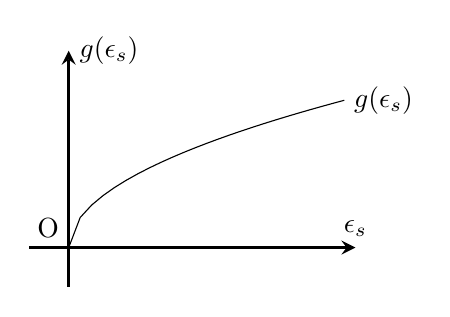
\begin{tikzpicture}
 \draw[->,>=stealth,very thick] (-0.5,0)--(pi+0.5,0)node[above]{$\epsilon_s$}; %x軸
 \draw[->,>=stealth,very thick] (0,-0.5)--(0,2.5)node[right]{$g(\epsilon_s)$}; %y軸
 \draw (0,0)node[above left]{O}; %原点
\draw[black,domain=0:3.5] plot(\x,{sqrt(\x)})node[right]{$g(\epsilon_s)$};
\end{tikzpicture}
  \label{ep12}
  \caption{$g(\epsilon_s)$は$\epsilon_s^{1/2}$に比例している.}
\end{figure}
%















%
\subsection{ミクロカノニカル集団とBoltzmannの原理}
一定の体積$V$をもち,外界と熱的・力学的相互作用のない「孤立系」を考える.この系は粒子数$N$,体積$V$,エネルギー$E$が指定される.このような熱力学系の集合はミクロカノニカル集団と呼ばれている.この熱力学系に対する熱力学ポテンシャル(状態量)はエントロピー$S$である.孤立系のエントロピー$S$は常に増加するか,または一定である.\\
 統計力学と熱力学を結び付けるために,新たな関係式を原理的に導入する.これはBoltzmannによってはじめて提唱されたもので,Boltzmannの原理と呼ばれている.
%
%
\begin{itembox}[l]{Boltzmannの原理}
実現可能な微視的状態数$W$とエントロピー$S$は次の関係式によって,与えられる.
\be\label{boltz}
S=k_{{\rm B}}\ln{W}
\ee
ここで$k_{\rm{B}}$はボルツマン定数と呼ばれている.
\end{itembox}
この関係式はマクロの量$S$とミクロな量$W$をつないでいる.\\
 孤立系のエントロピー$S$は非減少的な量であるから,系のエントロピーは可能な限り増大する.したがって,エントロピー$S$,つまり,式(\ref{boltz})が最大となるとき,熱平衡状態となる.このこと「エントロピー最大原理」として定式化しよう.
 %
%
\begin{itembox}[l]{エントロピー最大原理}
孤立系の平衡状態で非拘束変数$W$のとる値は,$W$が取りうる値の中で,全エントロピーを最大化するものに等しい.
\end{itembox}





%
\subsection{エントロピーと最大化の方法}
(\ref{boltz})を用いて,エントロピーを書き直していく.$s$番目の一つのセルについて(\ref{b1})だけのばらまき方があった.これらは独立事象であるから,全体のばらまき方は,これらの積をつくり
\be\label{s1}
W=\prod_{s}W_s
=\prod_{s}
\frac{(N_s+M_s-1)!}{N_s!(M_s-1)!}
\ee
と表される.(\ref{boltz})へ(\ref{s1})を代入する.そして,Stirlingの近似式$\ln{N!}\sim N\ln N-N$を使い,$N_s,M_s\gg1$であることを考慮すると,エントロピー$S$は
\begin{align}\label{s2}
\frac{S}{k_{{\rm{B}}}}&=\ln{W}=\ln
\left[\prod_{s}
\frac{(N_s+M_s-1)!}{N_s!(M_s-1)!}
\right]
\sim\ln
\left[\prod_{s}
\frac{(N_s+M_s)!}{N_s!(M_s)!}
\right]
\nn[10pt]
%
&\sim\displaystyle\sum_{s}[(N_s+M_s)\ln(N_s+M_s)
-(N_s+M_s)-N_s\ln{N_s}+N_s-M_s\ln{M_s}+M_s
]\nn[10pt]
%
&=\displaystyle\sum_{s}[(N_s+M_s)\ln(N_s+M_s)
-N_s\ln{N_s}-M_s\ln{M_s}
]
\end{align}
となる.\\
 孤立系で全粒子数$N$とエネルギー$E$については拘束条件
\be\label{N}
N=\displaystyle\sum_sN_s
\ee
\be\label{E}
E=\displaystyle\sum_s\epsilon_sN_s
\ee
を満たさなければならない.\\
 エントロピーの表式(\ref{boltz})における微視的状態数$W$は任意であり,このままでは使えない.だから,「何らかの方法」で平衡状態の状態数$W_{\rm{eq}}$を決める必要がある.エントロピー最大原理に従うと,この系の熱平衡状態は拘束条件(\ref{N}),(\ref{E})の条件下で,(\ref{s2})を最大化することにより得られる.このような最大化問題は「ラグランジュの未定乗数法」によって求めることができる.つまり,$\alpha$,$\beta$を「ラグランジュの未定乗数」として,関数
\be\label{s3}
f\equiv\frac{S}{k_{{\rm{B}}}}+\alpha\left(N-\displaystyle\sum_sN_s\right)+\beta\left(E-\displaystyle\sum_s\epsilon_sN_s\right)
\ee
の最大化を考えればよい.この$f$が拘束条件の条件下で最大値をとるための必要条件は
\be
\frac{\partial f}{\partial N_s}
=
\frac{1}{k_{{\rm{B}}}}\frac{\partial S}{\partial N_s}
-\alpha
-\beta\epsilon_s
=0
\ee
である.(\ref{s2})の$N_s$についての偏微分を計算し,
\begin{align}\label{s4}
\frac{1}{k_{{\rm{B}}}}\frac{\partial S}{\partial N_s}
&=\frac{\partial }{\partial N_s}
\displaystyle\sum_{s}[(N_s+M_s)\ln(N_s+M_s)
-N_s\ln{N_s}-M_s\ln{M_s}
]\\[10pt]
%
&=\ln(N_s+M_s)+1
-\ln{N_s}-1
=\ln(N_s+M_s)-\ln{N_s}=\ln\frac{N_s-M_s}{N_s}
\end{align}
まとめると,
\be
\frac{\partial f}{\partial N_s}
=
\ln\frac{N_s-M_s}{N_s}
-\alpha
-\beta\epsilon_s
=0
\ee
となる.よって,この最大化問題の解は
\be\label{s5}
\ln\frac{N_s-M_s}{N_s}=
\alpha
+\beta\epsilon_s,\ \ \ \ \ 
N_s=\frac{1}{e^{\alpha+\beta\epsilon_s}-1}M_s
\ee
と求まる.








%
\subsection{Bose-Einstein分布}
$N$粒子気体に対する熱力学第一法則
\be\label{thm}
dU=TdS-PdV+\mu dN
\ee
を使って,$\alpha,\beta$を求めよう.ここで,$T$は熱力学的絶対温度,$P$は圧力,$\mu$は化学ポテンシャルである.ここでは体積$V$が一定の場合を考えているので,
\be\label{thm1}
dU=TdS+\mu dN
\ee
となる.
これを
\be\label{thm2}
dS=\frac{1}{T}(dU-\mu dN)
\ee
と書き直す.
\be
\frac{\partial S}{\partial N_s}=k_{\rm{B}}\alpha+k_{\rm{B}}\beta\epsilon_s
\ee
\begin{align}
dS&=\displaystyle\sum_s\frac{\partial S}{\partial N_s}dN_s
=k_{\rm{B}}\displaystyle\sum_s(\alpha+\beta\epsilon_s)dN_s\\[10pt]
&=k_{\rm{B}}(\beta dU+\alpha dN)=k_{\rm{B}}\beta dU+k_{\rm{B}}\alpha dN
\end{align}
となる.ここで,$dN=\displaystyle\sum_sdN_s,dU=\displaystyle\sum_s\epsilon_sdN_s$を用いた.上式と(\ref{thm2})を比較すれば,
\begin{align}
\beta&=\frac{1}{k_{\rm{B}} T}\\[5pt]
\alpha&=-\beta\mu
\end{align}
解(\ref{s5})へ$\alpha$を代入し,$f_{\rm {BE}}(\epsilon_s)\equiv N_s/M_s$とおけば,Bose-Einstein分布
\be
\fbox{$
f_{\rm {BE}}(\epsilon_s)=\dfrac{1}{e^{\beta(\epsilon_s-\mu)}-1}
$}
\ee
を得る.この分布の意味を述べよう.この分布は1粒子状態$s$を占有する平均粒子数という物理的意味をもつ.














%
\section{グランドカノニカル集団}
\subsection{グランドカノニカル分布と大分配関数}
一つの孤立系を着目系と大きな外部系の二つに分ける.つまり,図\ref{g5}のように,(エネルギー$E$,粒子数$N$で指定される)着目系が,熱・粒子浴という大きな外部系とエネルギーと粒子の交換を許されている場合を考える.このように,外部との間に,熱に加えて粒子のやり取りがある系を「開放系」という.これで巨視的な状態として化学ポテンシャル$\mu$,体積$V$,温度$T$を指定したことになる.この系に対する集団はグランドカノニカル集団と呼ばれる.\\
%
 \begin{figure}[H]
 \centering
\includegraphics[width=6cm,height=4cm]{file/basic_st/fig/bo6.png}
  \caption{大きな外部系とエネルギーと粒子のやり取りをする着目系}
  \label{g6}
\end{figure}




上の設定において,着目系の粒子数$N$を一つ選ぶ,またそれに対応するエネルギー固有状態$i=1,2,\ldots,n_N$を一つ固定する.着目系がある粒子数が$N$のとき,エネルギー固有状態$i$をとる確率は,
\be
P^{(N)}_i=\frac{1}{{\it{\Xi}}}\exp\Bigl[
-\beta(E_i^{(N)}-\mu N)
\Bigr]
\ee
ここで,$E_i^{(N)}$は粒子数が$N$のときの,エネルギー固有値である.また,${\it{\Xi}}$は大分配関数と呼ばれており,次式で与えられる:
\be
{\it{\Xi}}=
\displaystyle\sum_N
\displaystyle\sum_i
\exp\Bigl[
-\beta(E_i^{(N)}-\mu N)
\Bigr]
\ee
上の二式から分かる通り,確率$P^{(N)}_i$は温度$T$と化学ポテンシャル$\mu$をパラメータとして含んでいる.



%
\subsection{グランドカノニカル集団の熱力学ポテンシャル}
グランドカノニカル集団に属する系の熱力学ポテンシャルはグランドポテンシャルと呼ばれており,次式で表される:
\be
{\it\Omega}(T,V,\mu)=-k_{\rm{B}} T\ln{{\it{\Xi}}}
\ee
これは大分配関数${\it{\Xi}}$と熱力学量であるグランドポテンシャル${\it\Omega}$を結ぶ公式である.\\
 グランドポテンシャル${\it\Omega}$の微小変化が
\be
d{\it\Omega}=-SdT-PdV-Nd\mu
\ee
と表されることを用いれば,エントロピー$S$,圧力$P$,粒子数$N$は次の熱力学関係式から得ることができる:
\be
\left(
\frac{\partial{\it\Omega}}{\partial T}
\right)_{V,\mu}
=-S,\ \ \ 
\left(
\frac{\partial{\it\Omega}}{\partial V}
\right)_{T,\mu}
=-P,\ \ \ 
\left(
\frac{\partial{\it\Omega}}{\partial \mu}
\right)_{T,V}
=-N
\ee


\subsection{バルク極限(熱力学的極)に関する注意点}
グランドポテンシャルの関係式
\be
{\it\Omega}(T,V,\mu)=-k_{\rm{B}} T\ln{{\it{\Xi}}}
\ee
は系の熱的な変化に対して,グランドポテンシャル${\it\Omega}$と大分配関数の対数$\ln{{\it{\Xi}}}$の同等性を表しているに過ぎない.他の粒子数や体積に関する変化に対しては,バルク極限(熱力学的極限)が保たれている範囲でのみこの関係式の正当性が成り立つ.バルク極限とは次の条件である:
\be
N\to\infty,\ \ \ \ 
V\to\infty,\ \ \ \ 
\frac{N}{V}=n\text{(粒子数密度)}=\text{一定}
\ee
すなわち,本来は単位体積当たりのグランドポテンシャル
\be
\frac{{\it\Omega}(T,V,\mu)}{V}=\omega(T,V,\mu)
\ee
として,次のように定式化する必要がある:
\be
\omega(T,V,\mu)
\equiv
-\lim_{V\to\infty}\frac{k_{\rm{B}} T}{V}\ln{{\it{\Xi}}},\ \ \ \ 
\text{ただし}
N\to\infty,\ \ \ \ 
\frac{N}{V}=n\text{(粒子数密度)}=\text{一定}
\ee